\documentclass[sigconf,nonacm]{acmart}

\usepackage{booktabs}
\usepackage{array}
\usepackage{tikz}
\usepackage{pgfplots}
\pgfplotsset{compat=1.18}
\usetikzlibrary{arrows.meta,positioning}
\newcolumntype{P}[1]{>{\raggedright\arraybackslash}p{#1}}

\settopmatter{printacmref=false}
\setcopyright{none}

\begin{document}

\title{Filipino Adaptation of OmniVoice for Voice Cloning and Text-to-Speech: A Pilot Study}

\author{Duncan F. Bandojo}
\author{Kristina Cassandra D. Bognot}
\author{Gwyneth Anne M. Gabales}
\author{Michael Lannz M. Salalima}
\author{Joanna Mae R. Salvador}
\affiliation{%
  \institution{Polytechnic University of the Philippines}
  \city{Manila}
  \country{Philippines}
}

\renewcommand{\shortauthors}{Bandojo et al.}

\begin{abstract}
This pilot study asks whether Filipino-specific fine-tuning improves OmniVoice, a pretrained massively multilingual zero-shot text-to-speech and voice cloning model. OmniVoice already supports Filipino, but its language table reports only 7.71 hours of Filipino in the original multilingual training mixture. We prepare a cleaned 39.8-hour Filipino read-speech corpus from the UP-DSP Philippine Languages Database, tokenize the audio with the Higgs Audio tokenizer, fine-tune the pretrained checkpoint on free Kaggle T4 GPUs, and evaluate generated speech on a 4,322-utterance speaker-disjoint test set using word error rate (WER), objective speaker similarity (SIM-o), and UTMOS. Four systems are compared: the base model and three fine-tuned checkpoints that differ in learning rate, step count, and checkpoint-selection policy. The strongest checkpoint, selected by lowest development loss at step 4900 of a 1e-5 run, reduces WER from 22.55\% to 18.52\% (a 17.9\% relative reduction) while keeping SIM-o slightly above the base model. A 2000-step run at a lower learning rate instead increased WER above the base model despite achieving the highest SIM-o. Filipino fine-tuning can therefore improve intelligibility under limited compute, but the gains depend strongly on checkpoint selection and cannot be judged from training loss or speaker similarity alone.
\end{abstract}

\begin{CCSXML}
<ccs2012>
<concept>
<concept_id>10010147.10010178.10010179</concept_id>
<concept_desc>Computing methodologies~Natural language processing</concept_desc>
<concept_significance>500</concept_significance>
</concept>
<concept>
<concept_id>10010147.10010257.10010293.10010294</concept_id>
<concept_desc>Computing methodologies~Neural networks</concept_desc>
<concept_significance>300</concept_significance>
</concept>
</ccs2012>
\end{CCSXML}

\ccsdesc[500]{Computing methodologies~Natural language processing}
\ccsdesc[300]{Computing methodologies~Neural networks}

\keywords{text-to-speech, voice cloning, Filipino, low-resource languages, transfer learning, OmniVoice, Philippine Languages Database}

\maketitle

\section{Introduction}

Voice cloning and text-to-speech (TTS) systems synthesize speech from written text and, in zero-shot voice cloning settings, imitate the voice of a reference speaker from a short audio prompt. Recent neural speech generation systems rely on pretrained multilingual models, discrete audio tokenizers, and generative modeling strategies to support many languages and speakers without training a new model for every use case \cite{valle,voicebox,maskgct,omnivoice}. These systems matter for accessibility, education, narration, localization, and language-learning applications.

Filipino is a major language in the Philippines, but open Filipino voice cloning workflows remain less developed than English-centered systems. Training a Filipino model from scratch would require data and compute far beyond a course-scale project. A more practical path is transfer learning \cite{transferlearning}: start from an existing multilingual TTS model and fine-tune it on a curated Filipino dataset.

OmniVoice is a suitable base model for this approach because it is open source, supports more than 600 languages, and includes Filipino with language ID \texttt{fil} \cite{omnivoice}. Broad coverage, however, does not guarantee strong language-specific quality. OmniVoice reports 7.71 hours of Filipino in its multilingual training mixture, while the UP-DSP Philippine Languages Database (PLD) holds 48:56:36 of Filipino speech \cite{pld}. The gap this study addresses is therefore not missing Filipino support; it is that Filipino-specific performance may remain limited because Filipino is a small fraction of the original training data, and a curated corpus with roughly four times more usable Filipino training speech is available to close that gap.

The machine learning problem is: given a pretrained multilingual voice cloning model and a curated Filipino speech-text corpus, determine whether supervised fine-tuning improves Filipino generated speech compared with the original pretrained checkpoint. The main research question follows directly: how much does Filipino-specific fine-tuning improve OmniVoice for Filipino TTS and voice cloning across intelligibility, naturalness, and speaker-similarity metrics?

To answer it, the study makes the following contributions:

\begin{enumerate}
  \item a cleaned, speaker-disjoint Filipino read-speech dataset (42,276 utterances, 39.8 hours) prepared from PLD in the JSONL and tokenized WebDataset format OmniVoice expects;
  \item a reproducible fine-tuning workflow for the pretrained \texttt{k2-fsa/OmniVoice} checkpoint that fits free Kaggle T4 GPU limits, with all runs tracked in Weights and Biases \cite{wandb};
  \item a controlled comparison of the base model and three fine-tuned checkpoints, evaluated on the full held-out test split with WER, SIM-o, and UTMOS;
  \item an error and trade-off analysis explaining which fine-tuning configuration helps, which hurts, and why checkpoint selection matters.
\end{enumerate}

The study is limited to Filipino read speech from PLD. It does not train a model from scratch, evaluate other Philippine languages, or claim commercial readiness. Evaluation is objective and automatic; human listening evaluation is a recommended next step. Kaggle's free T4 environment constrains model size, training steps, batch size, and checkpoint retention throughout.

\section{Related Work}

Voice cloning is a specialized form of TTS where the system must generate the requested content while preserving speaker identity from a reference prompt \cite{voicecloningsurvey}. Recent work has shifted from speaker-specific systems toward large pretrained speech generation models. VALL-E demonstrated neural codec language modeling for zero-shot TTS by generating discrete audio codec tokens conditioned on text and a short acoustic prompt \cite{valle}. Voicebox extended multilingual speech generation and text-guided speech editing at scale \cite{voicebox}. MaskGCT and F5-TTS reflect a broader move toward efficient non-autoregressive or masked generation \cite{maskgct,f5tts}.

OmniVoice is the model most directly connected to this study. It is a massively multilingual zero-shot TTS system with a diffusion language model-style masked-token prediction process \cite{omnivoice}. Instead of predicting semantic tokens first and then generating acoustic tokens, OmniVoice directly maps text and conditioning signals into multi-codebook acoustic tokens. It uses the Higgs Audio tokenizer for 8-codebook acoustic representation and waveform reconstruction \cite{higgsaudio}. These design choices make it practical to fine-tune an existing pretrained checkpoint rather than build a new Filipino speech generator from scratch.

The UP-DSP Philippine Languages Database is the primary data source. Cajote et al. \cite{pld} describe PLD as a multilingual speech corpus for Philippine spoken languages, covering Filipino, English, Cebuano, Kapampangan, Hiligaynon, Ilokano, Bikolano, Waray, and Tausug. The Filipino subset provides the paired speech and transcript files that supervised TTS fine-tuning requires.

Evaluation in zero-shot TTS usually separates intelligibility, speaker preservation, and naturalness. WER or CER measures intelligibility through an ASR model \cite{whisper,levenshtein}, speaker-embedding cosine similarity measures objective speaker preservation \cite{ecapatdnn,wavlm}, and UTMOS estimates naturalness \cite{utmos}. OmniVoice and Voicebox report these same metric families \cite{omnivoice,voicebox}; this study adapts that evaluation logic to Filipino fine-tuning.

\section{Methodology}

Figure~\ref{fig:pipeline} shows the five stages of the workflow: dataset preparation, audio tokenization, fine-tuning, matched inference, and objective evaluation.

\begin{figure}[t]
  \centering
  \small
  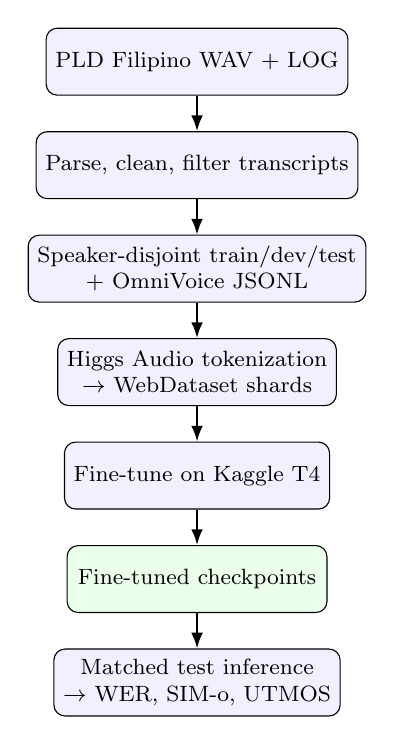
\begin{tikzpicture}[
    node distance=0.45cm and 0.5cm,
    box/.style={draw, rounded corners, align=center, minimum height=0.85cm, minimum width=3.3cm, fill=blue!6, font=\footnotesize},
    outputbox/.style={draw, rounded corners, align=center, minimum height=0.85cm, minimum width=3.3cm, fill=green!8, font=\footnotesize},
    arrow/.style={-{Latex[length=2mm]}, thick}
  ]
    \node[box] (raw) {PLD Filipino WAV + LOG};
    \node[box, below=of raw] (parse) {Parse, clean, filter transcripts};
    \node[box, below=of parse] (split) {Speaker-disjoint train/dev/test\\+ OmniVoice JSONL};
    \node[box, below=of split] (tokens) {Higgs Audio tokenization\\$\rightarrow$ WebDataset shards};
    \node[box, below=of tokens] (train) {Fine-tune on Kaggle T4};
    \node[outputbox, below=of train] (ckpt) {Fine-tuned checkpoints};
    \node[box, below=of ckpt] (eval) {Matched test inference\\$\rightarrow$ WER, SIM-o, UTMOS};

    \draw[arrow] (raw) -- (parse);
    \draw[arrow] (parse) -- (split);
    \draw[arrow] (split) -- (tokens);
    \draw[arrow] (tokens) -- (train);
    \draw[arrow] (train) -- (ckpt);
    \draw[arrow] (ckpt) -- (eval);
  \end{tikzpicture}
  \caption{Fine-tuning and evaluation pipeline.}
  \label{fig:pipeline}
\end{figure}

\subsection{Dataset and Pre-processing}

The dataset is the Filipino subset of the UP-DSP Philippine Languages Database, released through Mozilla Data Collective under a CC-BY-NC-4.0 license. It consists of WAV audio files and LOG transcript files. The PLD paper reports 135 speakers, 52,879 utterances, 48:56:36 total duration, and a 3.58-second average utterance for the Filipino subset \cite{pld}.

Only read or prompted Filipino speech was used. Spontaneous speech was excluded because a speaker's free response may not match the displayed prompt, which raises transcript-audio mismatch risk for supervised TTS. The preparation script parses PLD folders, matches WAV files to LOG transcript entries, filters unsuitable rows, and writes OmniVoice-compatible JSONL manifests. Each row contains an utterance ID, relative audio path, transcript text, and language ID:

\begin{verbatim}
{"id":"0000.110816.021250.0001",
 "audio_path":"wavs/0000/....0001.wav",
 "text":"manugang",
 "language_id":"fil"}
\end{verbatim}

The filtering rules were intentionally conservative: spontaneous prompt sources were dropped, transcripts containing parentheses or digits were excluded, unreadable or zero-byte WAV files were removed, only clips between 1.0 and 15.0 seconds were kept, and transcript whitespace was lightly normalized. Speakers were split disjointly across train, development, and test sets so that no test voice appears in training. Table~\ref{tab:prepared-split} shows the resulting splits.

\begin{table}[t]
  \centering
  \caption{Prepared Filipino dataset splits (speaker-disjoint).}
  \label{tab:prepared-split}
  \begin{tabular}{lrrrr}
    \toprule
    Split & Samples & Percent & Hours & Speakers \\
    \midrule
    Train & 33,448 & 79.12\% & 31.90 & 103 \\
    Development & 4,506 & 10.66\% & 3.71 & 13 \\
    Test & 4,322 & 10.22\% & 4.17 & 13 \\
    \midrule
    Total & 42,276 & 100.00\% & 39.77 & 129 \\
    \bottomrule
  \end{tabular}
\end{table}

The cleaned corpus spans varied prompt domains. The largest read-speech sources are news sentences (4,330 clips), medical sentences (2,397), time expressions (1,973), common expressions (1,941), short stories (1,904), greetings (1,708), interrogatives (1,634), and Filipino proverbs or \textit{salawikain} (1,620). Many remaining sources are isolated-word prompts (names, cuisines, landmarks, ordinals), which explains the short average utterance length and matters later when interpreting prosody-related results.

The 31.9 training hours are roughly four times the 7.71 Filipino hours in OmniVoice's original training mixture, which is the quantitative basis for expecting fine-tuning to help.

\subsection{Audio Tokenization}

OmniVoice does not train on raw waveforms. Audio is resampled to 24 kHz and converted into discrete 8-codebook acoustic token sequences with the Higgs Audio V2 tokenizer\footnote{\texttt{eustlb/higgs-audio-v2-tokenizer} on the Hugging Face Hub.} \cite{higgsaudio}, then stored in WebDataset shards referenced through \texttt{data.lst} manifests. Tokenization is expensive on free GPUs, so the tokenized full dataset was saved once as a Kaggle dataset artifact and reused across all training runs. Text needs no feature engineering beyond keeping the Filipino transcript and the \texttt{fil} language ID.

\subsection{Fine-Tuning Setup}

All runs fine-tune the pretrained \texttt{k2-fsa/OmniVoice} checkpoint, whose language model component is \texttt{Qwen/Qwen3-0.6B}, inside Kaggle T4 notebooks. Weights and Biases tracked configurations, losses, checkpoints, generated examples, and evaluation summaries \cite{wandb}; the consolidated report is available online.\footnote{\url{https://wandb.ai/duncanb013-polytechnic-university-of-the-philippines/OmniVoice-PLD-Filipino/reports/OmniVoice-PLD-Filipino-finetuning--VmlldzoxNjk0ODkyMg?accessToken=ktcztpc3ocu4gmtctis13mdubb82ec1r4rnyuxdta56tts4z5j4f965olbm0v5ka}} Table~\ref{tab:shared-config} lists the shared configuration.

\begin{table}[t]
  \centering
  \caption{Shared training configuration across all fine-tuning runs.}
  \label{tab:shared-config}
  \small
  \begin{tabular}{P{0.42\linewidth}P{0.46\linewidth}}
    \toprule
    Field & Value \\
    \midrule
    Base model & \texttt{k2-fsa/OmniVoice} \\
    LLM path & \texttt{Qwen/Qwen3-0.6B} \\
    Audio tokenizer & Higgs Audio V2 \\
    Audio codebooks / vocab & 8 / 1025 (mask ID 1024) \\
    Precision / attention & FP16 / SDPA \\
    Batch tokens & 1024 \\
    Gradient accumulation & 8 \\
    Max batch size & 4 \\
    Sample tokens (min--max) & 50--1200 \\
    Optimizer & AdamW, weight decay 0.01 \\
    Max gradient norm & 1.0 \\
    LR schedule & cosine decay, 1\% warmup \\
    Loss & weighted cross-entropy on masked acoustic tokens \\
    Codebook loss weights & [8, 8, 6, 6, 4, 4, 2, 2] \\
    Mask ratio range & [0.0, 1.0] \\
    Prompt ratio range & [0.0, 0.3] \\
    Drop condition ratio & 0.1 \\
    Seed & 42 \\
    \bottomrule
  \end{tabular}
\end{table}

The loss is OmniVoice's own training objective. OmniVoice is a single-stage non-autoregressive model trained with a discrete masked diffusion objective \cite{omnivoice}: random target audio-token positions are replaced by the mask token, and the model recovers the original token IDs only at those positions, conditioned on text, language, prompt audio, and unmasked target tokens. Our runs implement this as weighted cross-entropy over masked acoustic-token positions; text tokens, control tokens, prompt audio, and unmasked targets are excluded from the loss. The codebook weights [8, 8, 6, 6, 4, 4, 2, 2] emphasize lower codebooks, which carry coarser speech structure.

Three runs tested different adaptation regimes:

\begin{itemize}
  \item \textbf{FT-1000:} learning rate 2e-5 for 1000 steps; final step checkpoint. A short first run to test whether adaptation moves the metrics at all. Its development loss at step 1000 was 4.192.
  \item \textbf{FT-2000:} learning rate 5e-6 for 2000 steps; final step checkpoint. A more conservative update over more steps.
  \item \textbf{FT-4900:} learning rate 1e-5 for a 5000-step run with a development-loss-selected policy: the development set is evaluated at fixed intervals and a checkpoint is saved only when development loss improves. The lowest development loss, 4.162, occurred at step 4900.
\end{itemize}

The learning rates are deliberately lower than OmniVoice's large-scale pretraining setting because these runs update an already pretrained checkpoint on a much smaller corpus. The 1\% warmup gives 10, 20, and 50 warmup steps for the three runs respectively.

\subsection{Evaluation Design}

All systems were evaluated on the same held-out 4,322-utterance test split with identical manifests, inference parameters, and evaluator models, so differences between rows reflect the checkpoints rather than the pipeline.

For each test utterance, the model generates the target text while cloning a reference voice. The reference prompt is a \emph{different} utterance from the same test speaker (the next utterance from that speaker in the manifest), so the model never hears the target audio it must produce. Inference used 32 unmasking steps with batch size 2 on two T4 GPUs. The base model and the 1000-step checkpoint were measured in a first full evaluation run; a later run evaluated the 2000-step and 4900-step checkpoints and reused the base row, which is valid because the test split, manifests, inference parameters, and evaluator versions were unchanged.

Three objective metrics were computed with the OmniVoice evaluation modules and the \texttt{k2-fsa/TTS\_eval\_models} evaluator checkpoints:

\begin{itemize}
  \item \textbf{WER} (lower is better): generated audio is transcribed by Whisper-large-v3 \cite{whisper} with Tagalog as the decoding language, and the transcript is compared with the target text by edit distance \cite{levenshtein}:
  \begin{equation}
    \mathrm{WER} = \frac{S + D + I}{N} \times 100,
  \end{equation}
  where $S$, $D$, $I$ are substitutions, deletions, and insertions and $N$ is the number of reference words. WER is an ASR-mediated intelligibility estimate, not a direct human comprehension score.
  \item \textbf{SIM-o} (higher is better): cosine similarity between speaker embeddings of the reference prompt and the generated audio,
  \begin{equation}
    \mathrm{SIM\text{-}o}(r,g) =
    \frac{\mathbf{e}_r \cdot \mathbf{e}_g}
         {\lVert \mathbf{e}_r \rVert \lVert \mathbf{e}_g \rVert},
  \end{equation}
  using a WavLM-large ECAPA-TDNN speaker encoder \cite{wavlm,ecapatdnn}.
  \item \textbf{UTMOS} (higher is better): a learned mean-opinion-score predictor for naturalness \cite{utmos}, averaged over all generated test files.
\end{itemize}

\section{Results and Discussion}

\subsection{Objective Metric Comparison}

Table~\ref{tab:results-main} and Figure~\ref{fig:wer-chart} summarize the full-test-set comparison.

\begin{table}[t]
  \centering
  \caption{Full PLD Filipino test-set results. Lower WER is better; higher SIM-o and UTMOS are better. Bold marks the best value per column.}
  \label{tab:results-main}
  \small
  \setlength{\tabcolsep}{4pt}
  \begin{tabular}{lrrrr}
    \toprule
    Model & WER (\%) & $\Delta$WER & SIM-o & UTMOS \\
    \midrule
    Base OmniVoice & 22.55 & --- & 0.602 & \textbf{3.64} \\
    FT-1000 (2e-5) & 20.07 & $-$2.48 & 0.610 & 3.60 \\
    FT-2000 (5e-6) & 22.64 & $+$0.09 & \textbf{0.611} & 3.57 \\
    FT-4900 (1e-5, dev-selected) & \textbf{18.52} & $-$4.03 & 0.604 & 3.61 \\
    \bottomrule
  \end{tabular}
\end{table}

\begin{figure}[t]
  \centering
  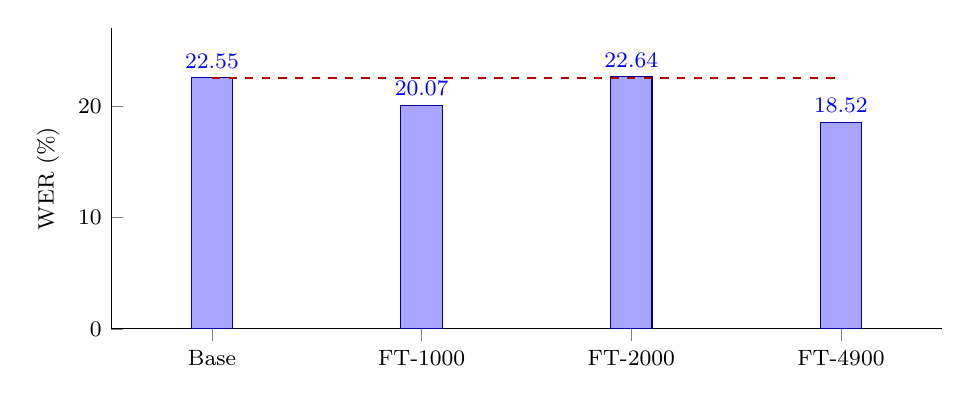
\begin{tikzpicture}
    \begin{axis}[
      ybar,
      bar width=15pt,
      width=\columnwidth,
      height=5.4cm,
      ylabel={WER (\%)},
      ymin=0, ymax=27,
      symbolic x coords={Base, FT-1000, FT-2000, FT-4900},
      xtick=data,
      nodes near coords,
      nodes near coords style={font=\footnotesize},
      enlarge x limits=0.16,
      axis lines*=left,
      tick label style={font=\footnotesize},
      label style={font=\footnotesize},
    ]
      \addplot+[fill=blue!35, draw=blue!60!black] coordinates {
        (Base,22.55) (FT-1000,20.07) (FT-2000,22.64) (FT-4900,18.52)
      };
      \draw[red!70!black, dashed, thick]
        (axis cs:Base,22.55) -- (axis cs:FT-4900,22.55);
    \end{axis}
  \end{tikzpicture}
  \caption{Test-set WER by system. The dashed line marks the base-model WER; only FT-1000 and FT-4900 fall below it.}
  \label{fig:wer-chart}
\end{figure}

The base model obtained 22.55\% WER, 0.602 SIM-o, and 3.64 UTMOS, confirming that OmniVoice is already a usable Filipino system before adaptation. FT-1000 improved WER to 20.07\% and raised SIM-o to 0.610, with a small UTMOS drop to 3.60, so even a short first run moved the model toward clearer Filipino output without losing the reference voice.

FT-2000, despite training twice as long at a lower learning rate, did not improve overall performance: it achieved the highest SIM-o (0.611) but its WER rose to 22.64\%, slightly worse than the base model. Speaker similarity alone is therefore not sufficient for selecting the strongest model; a voice cloning system must also say the intended words.

The strongest result came from FT-4900, the development-loss-selected checkpoint of the 1e-5 run. It reached 18.52\% WER, 4.03 absolute points below the base model and a 17.9\% relative reduction, while keeping SIM-o slightly above base (0.604) and UTMOS within 0.03 of the other fine-tuned checkpoints. It is the strongest overall checkpoint because it gives the largest intelligibility gain without a speaker-similarity or naturalness collapse.

\subsection{Error Analysis}

Table~\ref{tab:wer-counts-final} and Figure~\ref{fig:editops-chart} break WER into edit operations.

\begin{table}[t]
  \centering
  \caption{WER edit-operation counts on the full test set.}
  \label{tab:wer-counts-final}
  \small
  \begin{tabular}{lrrrr}
    \toprule
    Model & Ins. & Del. & Sub. & Words \\
    \midrule
    Base OmniVoice & 2,668 & 640 & 2,858 & 27,342 \\
    FT-1000 & 2,439 & 598 & 2,452 & 27,354 \\
    FT-2000 & 3,115 & 586 & 2,492 & 27,354 \\
    FT-4900 & 2,045 & 603 & 2,417 & 27,354 \\
    \bottomrule
  \end{tabular}
\end{table}

\begin{figure}[t]
  \centering
  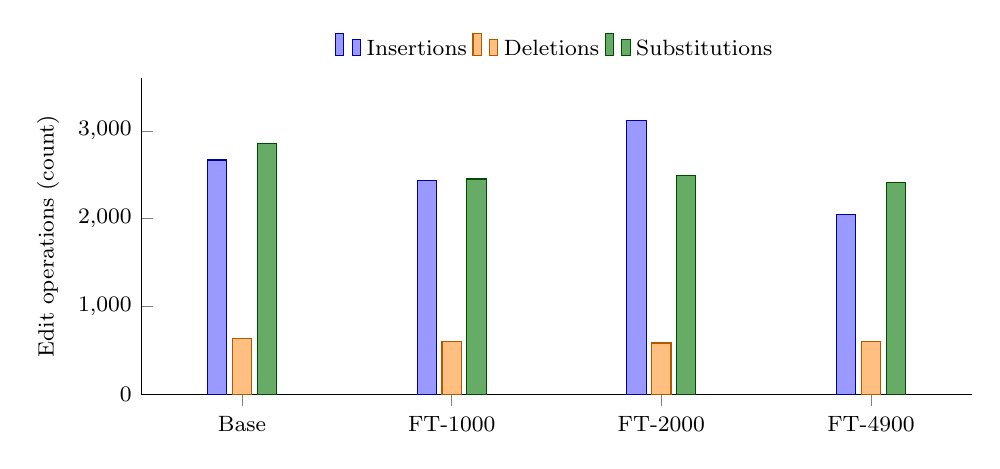
\begin{tikzpicture}
    \begin{axis}[
      ybar,
      bar width=7pt,
      width=\columnwidth,
      height=5.6cm,
      ylabel={Edit operations (count)},
      ymin=0, ymax=3600,
      symbolic x coords={Base, FT-1000, FT-2000, FT-4900},
      xtick=data,
      enlarge x limits=0.16,
      axis lines*=left,
      legend style={font=\footnotesize, at={(0.5,1.02)}, anchor=south, legend columns=3, draw=none},
      tick label style={font=\footnotesize},
      label style={font=\footnotesize},
    ]
      \addplot+[fill=blue!40, draw=blue!60!black] coordinates {
        (Base,2668) (FT-1000,2439) (FT-2000,3115) (FT-4900,2045)};
      \addplot+[fill=orange!50, draw=orange!70!black] coordinates {
        (Base,640) (FT-1000,598) (FT-2000,586) (FT-4900,603)};
      \addplot+[fill=green!45!black!60, draw=green!30!black] coordinates {
        (Base,2858) (FT-1000,2452) (FT-2000,2492) (FT-4900,2417)};
      \legend{Insertions, Deletions, Substitutions}
    \end{axis}
  \end{tikzpicture}
  \caption{Edit operations per system. FT-4900 wins mainly by cutting insertions; FT-2000 loses its gains to an insertion increase.}
  \label{fig:editops-chart}
\end{figure}

The edit counts explain the ranking. Compared with the base model, FT-4900 reduced insertions from 2,668 to 2,045 and substitutions from 2,858 to 2,417, while deletions stayed near the base level. Its improvement comes from producing fewer extra words and fewer wrongly recognized words. FT-2000 reduced deletions and substitutions but raised insertions to 3,115, and that single increase was large enough to push its total WER above the base model. A fine-tuned model can therefore improve one error type while worsening another, which is why aggregate WER must be read together with its components.

\subsection{Development Loss versus Downstream Metrics}

Development loss was used to monitor training and select checkpoints, and the relationship to downstream quality turned out to be useful but imperfect. The dev-loss-selected FT-4900 run did produce the lowest WER, and its best development loss (4.162) was lower than FT-1000's (4.192). But FT-1000 already delivered most of a useful WER gain from a much shorter run, and FT-2000's high SIM-o paired with worse WER shows that no single training-time signal predicts the full metric pattern. Development loss is a good checkpoint-selection heuristic; it still must be validated with downstream audio metrics before declaring a winner.

The configuration choices that mattered most were the combination of longer training, the repository-aligned 1e-5 learning rate, and saving a development-loss-selected checkpoint instead of only the last step. The FT-2000 result shows that simply lowering the learning rate is not automatically safer under the same compute budget.

\subsection{Practical Findings}

Several workflow-level findings emerged. Reusing tokenized audio as a Kaggle dataset artifact was essential because token extraction is expensive and would otherwise be repeated every run. The conservative T4 recipe (FP16, SDPA attention, small per-forward token batches, gradient accumulation) made training feasible at all; a 1000-step run completed in roughly one hour. Full-test evaluation is slow, so reusing the base-model row across evaluation notebooks is practical when the evaluation setup is frozen. Finally, the strongest model should be chosen by a coherent metric pattern rather than a single number: WER is primary here because intelligibility is the research question, while SIM-o and UTMOS guard against selecting a clearer model that damages voice similarity or naturalness.

\subsection{Limitations}

The completed comparison uses automatic metrics only. WER depends on the ASR model (Whisper-large-v3 decoding Tagalog), so it estimates intelligibility as that ASR system hears it; SIM-o depends on the speaker encoder; and UTMOS is a learned MOS predictor, not a listening survey. The corpus is Filipino read speech with many short, isolated-word prompts, so the results say little about spontaneous speech, long-form prosody, or other Philippine languages. Compute limits also restricted the number of hyperparameter runs, so the learning-rate comparison samples three points rather than a full sweep.

\section{Conclusion and Recommendations}

Filipino-specific fine-tuning can improve OmniVoice for Filipino TTS and voice cloning. The strongest evaluated checkpoint, FT-4900 (1e-5 learning rate, selected by lowest development loss), reduced WER from 22.55\% to 18.52\% while keeping SIM-o slightly above the base model. The improvement is real but conditional: FT-2000 shows that a fine-tuned checkpoint can also be worse than the base model on the primary metric, so fine-tuned models must be compared with downstream metrics rather than training loss, development loss, or speaker similarity alone.

Three directions follow. First, a Filipino listener study should validate whether the WER gain matches human judgments of pronunciation, intelligibility, naturalness, and speaker similarity; the automatic metrics used here are proxies for all four. Second, the training side should test more checkpoints around the 1e-5 learning rate, compare last-step and development-loss-selected policies systematically, and inspect generated audio where WER remains high. Third, the data side should build a verified subset of longer sentence-level utterances, since the current corpus is dominated by short prompts, and test whether sentence-level training data improves Filipino prosody. For demonstration and reporting, the recommended checkpoint is FT-4900.

\bibliographystyle{ACM-Reference-Format}
\bibliography{references}

\appendix

\section{Weights and Biases Training Curves}
\label{app:ct-wandb-curves}

The full interactive experiment report is available in the project's W\&B workspace (footnote in Section 3.3).

\begin{figure*}[t]
  \centering
  
\includegraphics[width=0.92\textwidth,keepaspectratio]{\detokenize{../../images/finetunes_training_loss_together.png}}
  \caption{Combined W\&B training-loss curves for the Filipino OmniVoice fine-tuning runs.}
  \label{fig:ct-finetunes-training-loss}
\end{figure*}

\section{Fine-Tuning Run Screenshots}
\label{app:ct-finetune-run-screens}

\begin{figure*}[t]
  \centering
  
\includegraphics[width=0.92\textwidth,keepaspectratio]{\detokenize{../../images/step 1000 lr 2e-5.png}}
  \caption{W\&B run screenshot for the 1000-step fine-tuning run at learning rate 2e-5.}
  \label{fig:ct-step-1000-lr-2e-5}
\end{figure*}

\begin{figure*}[t]
  \centering
  
\includegraphics[width=0.92\textwidth,keepaspectratio]{\detokenize{../../images/step 2000 lr 5e-6.png}}
  \caption{W\&B run screenshot for the 2000-step fine-tuning run at learning rate 5e-6.}
  \label{fig:ct-step-2000-lr-5e-6}
\end{figure*}

\begin{figure*}[t]
  \centering
  
\includegraphics[width=0.92\textwidth,keepaspectratio]{\detokenize{../../images/step 5000 lr 1e-5.png}}
  \caption{W\&B run screenshot for the 5000-step fine-tuning run at learning rate 1e-5.}
  \label{fig:ct-step-5000-lr-1e-5}
\end{figure*}

\section{Generated Test Sample Tables}
\label{app:ct-sample-tables}

\begin{figure*}[t]
  \centering
  
\includegraphics[width=0.92\textwidth,keepaspectratio]{\detokenize{../../images/base_test_samples.png}}
  \caption{W\&B generated-test-samples table for the base OmniVoice model.}
  \label{fig:ct-base-test-samples}
\end{figure*}

\begin{figure*}[t]
  \centering
  
\includegraphics[width=0.92\textwidth,keepaspectratio]{\detokenize{../../images/finetune_1000_test_samples.png}}
  \caption{W\&B generated-test-samples table for the 1000-step fine-tuned checkpoint.}
  \label{fig:ct-finetune-1000-test-samples}
\end{figure*}

\begin{figure*}[t]
  \centering
  
\includegraphics[width=0.92\textwidth,keepaspectratio]{\detokenize{../../images/finetune_2000_test_samples.png}}
  \caption{W\&B generated-test-samples table for the 2000-step fine-tuned checkpoint.}
  \label{fig:ct-finetune-2000-test-samples}
\end{figure*}

\begin{figure*}[t]
  \centering
  
\includegraphics[width=0.92\textwidth,keepaspectratio]{\detokenize{../../images/finetune_5000_test_samples.png}}
  \caption{W\&B generated-test-samples table for the 5000-step fine-tuning run.}
  \label{fig:ct-finetune-5000-test-samples}
\end{figure*}

\end{document}
